\begin{frame}
    \frametitle{Background}
    \begin{block}{Stochastic Boolean Satisfiability (SSAT)}
        $\Qf=Q_1 x_1,\ldots,Q_n x_n.\pf$
        \pause
        \begin{itemize}
            \item $Q_1 x_1,\ldots,Q_n x_n$: quantification structure, $Q_i \in \{\random{p},\exists\}$ (\emph{prefix})
                  \pause
            \item $\pf$: quantifier-free formula over $\{x_1,\ldots,x_n\}$ (\emph{matrix})
        \end{itemize}
    \end{block}
    \pause
    \begin{block}{Computational Rules for Satisfying Probability}
        Let $x$ be the outermost variable in the prefix:
        \pause
        \begin{enumerate}
            \item[a)] $\spb{\top}=1$,
                  \pause
            \item[b)] $\spb{\bot}=0$,
                  \pause
            \item[c)] $\spb{\Qf}=\max\{\spb{\ncf{\Qf}{x}},\spb{\pcf{\Qf}{x}}\}$, if $x$ is quantified by $\exists$,
                  \pause
            \item[d)] $\spb{\Qf}=(1-p)\spb{\ncf{\Qf}{x}}+p\spb{\pcf{\Qf}{x}}$, if $x$ is quantified by $\random{p}$.
        \end{enumerate}
    \end{block}
\end{frame}

\begin{frame}
    \frametitle{Background}
    \begin{block}{Example: Computation of Satisfying Probability}
        \abovedisplayskip=0pt
        \begin{align*}
             & \Qf=\random{0.5} x_1, \exists y_1, \random{0.5} x_2, \exists y_2. \pf \\
             & \pf=(x_1 \lor \lnot y_1)
            (\lnot x_1 \lor y_1)
            (\lnot x_1 \lor \lnot x_2 \lor y_2)
            (x_1 \lor \lnot y_2)
            (x_2 \lor \lnot y_2)
        \end{align*}
    \end{block}\pause
    \begin{figure}
        \centering
        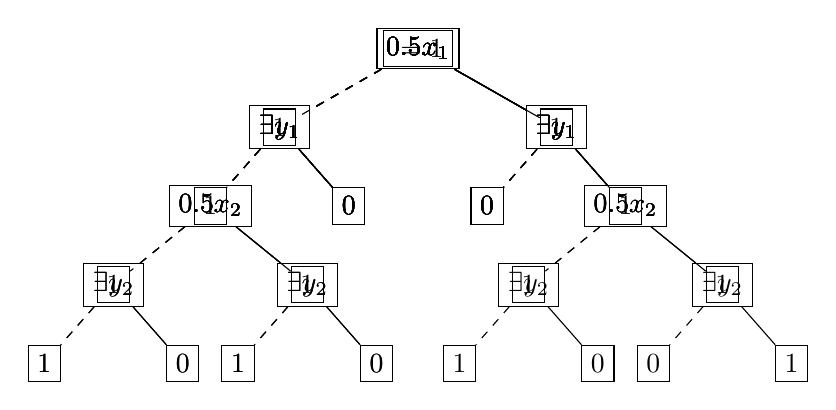
\begin{tikzpicture}[
                baseline,
                level distance=10mm,
                level 1/.style={sibling distance=10em},
                level 2/.style={sibling distance=5em},
                level 3/.style={sibling distance=7em},
                level 4/.style={sibling distance=5em},
                every node/.style={solid,draw},
                positive/.style={edge from parent/.style={solid,draw}},
                negative/.style={edge from parent/.style={dashed,draw}}]

            \action<2>{\node{$\random{0.5} x_1$};}
            \action<3>{\node{$\random{0.5} x_1$}
                child[negative]{node{$\exists y_1$}}
                child[positive]{node{$\exists y_1$}};}
            \action<4>{\node{$\random{0.5} x_1$}
                child[negative]{node{$\exists y_1$}
                        child[negative]{node{$\random{0.5} x_2$}}
                        child[positive]{node{$0$}}}
                child[positive]{node{$\exists y_1$}};}
            \action<5>{\node{$\random{0.5} x_1$}
                child[negative]{node{$\exists y_1$}
                        child[negative]{node{$\random{0.5} x_2$}}
                        child[positive]{node{$0$}}}
                child[positive]{node{$\exists y_1$}
                        child[negative]{node{$0$}}
                        child[positive]{node{$\random{0.5} x_2$}}};}
            \action<6>{\node{$\random{0.5} x_1$}
                child[negative]{node{$\exists y_1$}
                        child[negative]{node{$\random{0.5} x_2$}
                                child[negative]{node{$\exists y_2$}
                                        child[negative]{node{$1$}}
                                        child[positive]{node{$0$}}}
                                child[positive]{node{$\exists y_2$}
                                        child[negative]{node{$1$}}
                                        child[positive]{node{$0$}}}}
                        child[positive]{node{$0$}}}
                child[positive]{node{$\exists y_1$}
                        child[negative]{node{$0$}}
                        child[positive]{node{$\random{0.5} x_2$}}};}
            \action<7>{\node{$\random{0.5} x_1$}
                child[negative]{node{$\exists y_1$}
                        child[negative]{node{$\random{0.5} x_2$}
                                child[negative]{node{$\exists y_2$}
                                        child[negative]{node{$1$}}
                                        child[positive]{node{$0$}}}
                                child[positive]{node{$\exists y_2$}
                                        child[negative]{node{$1$}}
                                        child[positive]{node{$0$}}}}
                        child[positive]{node{$0$}}}
                child[positive]{node{$\exists y_1$}
                        child[negative]{node{$0$}}
                        child[positive]{node{$\random{0.5} x_2$}
                                child[negative]{node{$\exists y_2$}
                                        child[negative]{node{$1$}}
                                        child[positive]{node{$0$}}}
                                child[positive]{node{$\exists y_2$}
                                        child[negative]{node{$0$}}
                                        child[positive]{node{$1$}}}}};}
            \action<8>{\node{$\random{0.5} x_1$}
                child[negative]{node{$\exists y_1$}
                        child[negative]{node{$\random{0.5} x_2$}
                                child[negative]{node{$1$}}
                                child[positive]{node{$1$}}}
                        child[positive]{node{$0$}}}
                child[positive]{node{$\exists y_1$}
                        child[negative]{node{$0$}}
                        child[positive]{node{$\random{0.5} x_2$}
                                child[negative]{node{$1$}}
                                child[positive]{node{$1$}}}};}
            \action<9>{\node{$\random{0.5} x_1$}
                child[negative]{node{$\exists y_1$}
                        child[negative]{node{$1$}}
                        child[positive]{node{$0$}}}
                child[positive]{node{$\exists y_1$}
                        child[negative]{node{$0$}}
                        child[positive]{node{$1$}}};}
            \action<10>{\node{$\random{0.5} x_1$}
                child[negative]{node{$1$}}
                child[positive]{node{$1$}};}
            \action<11>{\node{$\spb{\Qf}=1$};}
        \end{tikzpicture}
    \end{figure}
\end{frame}

\begin{frame}
    \frametitle{Express Model-Counting Variants with SSAT}
    \begin{table}[t]
        \centering
        \begin{tabular}{c|c}
            Variant            & SSAT encoding                                                               \\
            \hline
            Unweighted         & $\random{0.5}x_1,\ldots,\random{0.5}x_n.\pf$                                \\
            Weighted           & $\random{p_1}x_1,\ldots,\random{p_n}x_n.\pf$                                \\
            Projected          & $\random{0.5}x_1,\ldots,\random{0.5}x_n,\exists y_1,\ldots,\exists y_m.\pf$ \\
            Maximum            & $\exists x_1,\ldots,\exists x_n,\random{0.5}y_1,\ldots,\random{0.5}y_m.\pf$ \\
            Weighted projected & $\random{p_1}x_1,\ldots,\random{p_n}x_n,\exists y_1,\ldots,\exists y_m.\pf$ \\
            Weighted maximum   & $\exists x_1,\ldots,\exists x_n,\random{p_1}y_1,\ldots,\random{p_m}y_m.\pf$ \\
        \end{tabular}
    \end{table}
\end{frame}

\begin{frame}
    \frametitle{Background}
    \begin{block}{Game-Theoretical Interpretation of SSAT}
        $\Qf=Q_1 x_1,\ldots,Q_n x_n.\pf$, $Q_i \in \{\random{p},\exists\}$
        \pause
        \begin{itemize}
            \item $\random{p}$: nondeterministic factors
                  \pause
            \item $\exists$: an agent who plays under uncertainty
                  \pause
            \item $\pf$: game matrix
                  \pause
            \item $\spb{\Qf}$: the maximum winning probability of the agent
                  \pause
            \item \alert{Skolem functions}: a winning/optimization strategy of the agent
        \end{itemize}
    \end{block}\pause
    \begin{block}{Example: Skolem Functions}
        \abovedisplayskip=0pt
        \belowdisplayskip=0pt
        \begin{align*}
             & \Qf=\random{0.5} x_1, \exists y_1, \random{0.5} x_2, \exists y_2. \pf \\
             & \pf=(x_1 \lor \lnot y_1)
            (\lnot x_1 \lor y_1)
            (\lnot x_1 \lor \lnot x_2 \lor y_2)
            (x_1 \lor \lnot y_2)
            (x_2 \lor \lnot y_2)
        \end{align*}
        \pause
        \begin{itemize}
            \item Variable $y_1$: $f_1(x_1)=x_1$; variable $y_2$: $f_2(x_1,x_2)=x_1 \land x_2$
        \end{itemize}
    \end{block}
\end{frame}